\documentclass[12pt]{article}

\usepackage[english]{babel}
\usepackage[utf8x]{inputenc}
\usepackage{amsmath}
\usepackage{enumitem}
\usepackage{graphicx}
\usepackage{ulem}
\usepackage{caption}
\usepackage{placeins}
\usepackage[usenames,dvipsnames]{color}
\usepackage[colorinlistoftodos]{todonotes}
\usepackage{listings}
\usepackage{fixltx2e}
\usepackage{scrpage2}
\usepackage{lastpage}
\clearscrheadfoot
\pagestyle{scrheadings}
\usepackage{glossaries}
\usepackage[
top    = 2.75cm,
bottom = 2.00cm,
left   = 2.50cm,
right  = 2.00cm]{geometry}
\setcounter{secnumdepth}{4}


\makeglossaries

\newglossaryentry{soa} {name=SOA, description={Service Oriented Architecture}}
\newglossaryentry{json} {name=JSON, description={Java Script Object Notation}}
\newglossaryentry{rest} {name=REST, description={Representational State Transfer}}
\newglossaryentry{aop} {name=AOP, description={Aspect Oriented Programming}}
\newglossaryentry{oop} {name=OOP, description={Object Oriented Programming}}
\newglossaryentry{bpm} {name=BPM, description={Business Process Management}}
\newglossaryentry{roi} {name=ROI, description={Return of Investment}}
\newglossaryentry{esb} {name=ESB, description={Enterprise Service Bus}}
\newglossaryentry{eai} {name=EAI, description={Enterprise Application Integration}}
\newglossaryentry{erp} {name=ERP, description={Enterprise Resource Planning}}

\begin{document}
\begin{titlepage}
\begin{center}
% Oberer Teil der Titelseite:

\includegraphics[width=0.75\textwidth]{images/logo}\\[1cm]    



\LARGE TGM - HTBLuVA Wien XX \\ IT Department  \\[1.5cm]

% Title
\rule{1.0\textwidth}{1mm}
{ \huge \bfseries \\[0.4cm]  \huge SOA, JSON and REST \\ \LARGE Dezsys-Elaboration \\[0.4cm] }

\rule{1.0\textwidth}{1mm}


% Author and supervisor
\noindent 
\vspace{5cm}

\begin{center}
\large
Authors: 
Siegel \textsc{Hannah} \&
Vogt \textsc{Andreas}
\end{center}

\vfill

% Bottom of the page
{\large \today}

\end{center}
\end{titlepage}

\tableofcontents


%HEADER AND FOOTER
\pagenumbering{arabic}
\ohead{\headmark}
\automark{section}
\ifoot{© Siegel,Vogt}
\ofoot{\pagemark ~of \pageref{LastPage}}

\newpage

\section{Introduction}
\subsection{Services}
In order to understand \gls{soa}, an very important concept is a \textit{Service}. \\
"Services are what you connect together using Web Services. A service is the endpoint of a connection. Also, a service has some type of underlying computer system that supports the connection offered. ",\cite{service1} \\ Furthermore, a Service has to have a clearly defined function and very often they should belong to one business process. It can be seen as an Interface which provides a specific function.\\ \\
\textbf{When do we speak of a service?}\\
"A service is also a unit of logic to which service-orientation has been applied to a meaningful extend. It's the application of service-orientation design principles that distingishues a unit of logic as a service compared to other units of logic that may exist solely as objects, components, Web services, REST services or cloud based systems",\cite[page 29]{grau} These patterns and principles are discussed in section \ref{sec:dp}. \\
A service contains it's clearly defined functionality, a description of this functionality and Basic-operations such as binding, selection, publication or discovery \cite[page 8]{soagoesreal}.  \\
Seen out of an more business related approach, they usually provide clear incident, problem, change, configuration, release, availibility and cost management - which helps to gain information and overview the services.
\subsection{SOA}
\textbf{Service-Oriented Computing}\\
"Service-oriented computing is an umbrella term that represents a distinct distributed computing platform. As such, it encompasses many things ,including its own design paradigm and design principles, design pattern catalogs, pattern languages, and a distinct architectural model, along with related concepts, technologies, and frameworks.",\cite[page 22]{grau}\\
\textbf{Service-Oriented Architcture}\\
%"A service-oriented architecture is essentially a collection of services. These services communicate with each other. The communication can involve either simple data passing or it could involve two or more services coordinating some activity. Some means of connecting services to each other is needed ",\cite{soaserviearch}. \\
"Service Oriented Architecture is a technology architectural model for service-oriented solutions with distinct characteristics in support of realizing service-orientation", \cite[page 27]{grau}. Service orientation means, that services of any kind are put into the center of the system, enabling flexible business process (re-)modelling due to a very high business process orientation and loose coupling of the services.\todo{bullshit.}\\  \\
"Service-oriented architecture (\gls{soa}) is an approach used to create an architecture based upon the use of services. Services (such as RESTful Web services) carry out some small function, such as producing data, validating a customer, or providing simple analytical services.",\cite{searchsoa} \gls{soa} is not a product or framework, it is a design approach or paradigm for good software design.
\\
SOA has it's underlying business functions provided as Services which can be used by all Application on a shared basis. The applications are using a middleware, for example an \gls{esb}, in order to access it's services. \\
\\Because \gls{soa} is using the technology of WebServices, it is quite platform independent. 
"It is important to view and position \gls{soa} and service-orientation as being neutral to any one technology platform. By doing so, you have the freedom to continually pursue the strategic goals associated with service-orientation computing by leveragng on-going service technology advancements.",cite[page 29]{grau} \\
\gls{soa} is often used as a newer approach to \gls{eai}. \cite{soaitwissen}
\\ \\
"One of the keys to SOA architecture is that interactions occur with loosely coupled services that operate independently. SOA architecture allows for service reuse, making it unnecessary to start from scratch when upgrades and other modifications are needed. This is a benefit to businesses that seek ways to save time and money.",\cite{searchsoa}. The aspect of an \gls{roi} is very important within the concept of \gls{soa}
\subsection{REST}
Rest stands for REpresentational State Transfer. It is a software architecture style consisting of guidelines and best practices 
for creating scalable web services.The main idea behind REST is that you are working with the HTTP protocol. Rest is basicly using HTTP verbs, GET, POST, PUT, DELETE and HEAD, in order to act on resources,represented by individual URIs(Uniform Resource Identifiers). 
A perk of those verbs is that they are mostly self-explanatory. REST is a lightweight alternative to mechanisms like RPC (Remote Procedure Calls) and Web Services (SOAP, WSDL, et al.)
\subsection{JSON}
"JSON (JavaScript Object Notation) is a lightweight data-interchange format. It is easy for humans to read and write. It is easy for machines to parse and generate. It is based on a subset of the JavaScript Programming Language, Standard ECMA-262 3rd Edition - December 1999. JSON is a text format that is completely language independent but uses conventions that are familiar to programmers of the C-family of languages, including C, C++, C sharp, Java, JavaScript, Perl, Python, and many others. These properties make JSON an ideal data-interchange language.",\cite{json}.

\section{Existing Problems}
\subsection{Historical Overview}
With the rise of computers, companies have started to invest into the new information technology during the second half of the 20 century.  Mostly, the first thing that has been bought were expensive mainframes, so that some processes could be done with more reliability. Naturally, employees have done some faults and they were not as efficient as computers. \\
Because of very expensive Hardware and Software which was by far not as evolved as it is today, the implementation of new technologies was quite slow. Computers and Mainframes were mostly used for industries like astronautics or applied researching and eventually even for automating processes such as book keeping. \\ 
These implementations were quite easy to implement and there was no need for any intercommunication between services.
\\ \\
In the early 80s, the whole industry changed. Suddenly, the personal computer (PC) made it possible to afford information technology on a large scale. Computers were not only used for difficult arithmetic operations but they started to be an everyday-life tool to improve the work-flow and the business processes in companies. \\
Many new kinds of technologies, ranging from OS with GUIs to the rise of the World Wide Web, were leading to an really fast expansion of information technology. \\ 
But with an higher demand on PCs, the demand for infrastructure rose as well. The need for computer specialist was higher than ever and every company had to invest a lot into their, mostly newly founded,  IT department. \\ \\
Because of an lack of know-how and systems that had the characteristics to change a lot, the implementation of all the services became a big challenge. Enterprises used a variety of customised applications, at least one for every type of service. \\ \\
\textbf{ODER:}
"Historically, many IT projects focused solely on building applications designed specifically to automate business process requirements that were current at theat time. This fulfilles immediate (tactical) needs, bit as mpre pf these single-purpose applications were delivered, it resulted in an IT enterprise filled with islands of logic and data reffered to as application \textit{silos}. As new business requirements would emerge, either new silos were created or integration channels between silos were established. As yet more business change arose, integration channels had to be augumented, even more silos had to be created, and soon the IT enterprise landscape became convoluted ad increasingly burdensome, expensive, and slow to evolve."\cite[page 522]{grau} 

\subsection{Problems}
Out of these systems, there are many problems that have eventually emerged. \\
First of all, systems like that are not really agile. Because changes and new technologies were inevitable, time consuming integrations had to be done. If these have simply not been, legacy systems emergered. These were often not remotly changeable. \\
Also, new challanges such as cloud computing and a more common globalization of Processes made it harder to stick to the old systems. \\
Because Applications were always providing some kind of service, but hardly seen like a service, they were not as easy reconfigurable and changeable. All the Applications need to communicate with each other and transmit data,so often a start topology was used. It then changed more and more into a Middleware, which had the benefit of only docking the Application to the Middleware once. Nowadays, mostly a bus system gets used, as described in section \ref{sec:esb}. \\
Due to compatibility concerns, IT-Infrastructure were often Vendor dependent. Therefore we often talk about an SAP-System, because mostly all the components have been bought from SAP, which decreases the agility and may increase the costs.\\
Furthermore, before \gls{soa}, Applications were not divided into processes, and therefore a \gls{bpm} was made difficult for both the management or the IT-department. \\
All these restriction lead to increased overall costs and an reduced \gls{roi}.
%TODO ausschmuecken? besser?
\section{SOA as an solution} 
"In many ways, service-orientation emerged in response to these problems. It is a paradigm that provides an alternative to project-specific, silo-based, and integrated application development by adamantly prioritizing the attainment of long-term, strategic business goals.",\cite[page 522]{grau} \\
The target state of service-orientation is to not have these traditional problems any more. In some cases, due to legacy systems or other problems this is not possible, but still \gls{soa} tries to realize it to whatever extend possible.
\\ \\
Service-orientation emerged as a formal method in support of achieving the following goals an benefits associated with service-oriented computing: \\
\begin{itemize}
\item Increased Intrinsic Interoperability
\item Increased Federation
\item Increased Vendor Diversification Options 
\item Increased Business and Technology Alignment
\item Increased \gls{roi}
\item Increased Organizational Agility
\item Reduced IT Burden
\end{itemize} \cite[page 23]{grau}
These strategic goals the are put into more low-level design principles. These goals are especially interesting not only to IT-staff members but also for a organization's management. \\
It is one step above \gls{eai} already and it combines important aspects of \gls{bpm}, \gls{oop} and \gls{aop} in it.
\subsection{Design Principles}
\label{sec:dp}
Because SOA is only an Design Paradigm and not a concrete implementation, service orientation Patterns and principles are used. The design paradigm consists of the following points:
\begin{enumerate}
\item Standardized Service contracts
\item Loosly coupled systems
\item Abstraction of Services
\item Reusability
\item Autonomity
\item Statelessness
\item Discoverability
\item Composability
\end{enumerate}\cite[page 25]{grau}
\subsubsection{Standardized Service contracts}
"A service contract expresses the technical interface of a service. ", cite[page 33]{grau} This means that there are interfaces which do contain the metadata to an service.  \\ If these services are implemented as a Webservice, for example, most commonly an description document in Form of an WSDL definition will be used, or an XML Schema. \\
The two approaches nowadays are either Top-Down (designing the service contracts at first and then implementing them) or Bottom-up(Building the contracts out of already existing services). \cite[page 151,152]{grau}
\\ \\
\textbf{REST}\\
"For REST services, capturing and communicating various aspects of resources can be necessary, such as the set of resources, relationships between resources, HTTP verbs allowed on resources and supported resource representation formats. Standards such as WADL(Web Application Description Language), can be used to satisfy the mandatory requirements. [..] Even the self-describing contract of HTTP verbs for a REST service establishes a standard-based service contract.", cite[page 151]{grau}
\\ \\
\textbf{SLAs} \\
Furthermore, A service contract will often be concluded in Human Readable documents. These are called Service Level Agreements (SLAs) and they often contain information like quality requirements or overall business information. %TODO grauslich.
\\ \\
\textbf{Generation Possibilities within Java} \\
"JAX-WS defines the wsimport tool, which takes an existing WSDL definintion as input to generate Java skeletons [..] Similarly, the wsgen tool generates WSDL from existing Java code.",\cite[page 151]{grau}
\\
%TODO service contract example!!!
\subsubsection{Loosly coupled systems}



\subsubsection{Abstraction of Services}
\subsubsection{Service Reusability}
The following are common design characteristics associated with reusable services:
\begin{itemize}
\item The service is defined by an agnositc functional context \\
	This means that an agnostic functional context is not specific to any one purpose and is therefore considered muli-purpose. It means, that it is idependent of the particular business process or the area of application.
\item The service logic is highly generic %TODO ???
\item The service can be used concurrently
\end{itemize}
In general, reusability is a very important design principle %TODO check
which gets used in normal \gls{oop} as well. \cite[page 140-150]{grau}
\subsubsection{Autonomity}
""
\subsubsection{Statelessness}
\subsubsection{Discoverability}
\subsubsection{Composability}
\subsection{SOA Manifesto }
The \gls{soa} Manifesto has been developed 2009, and it is quite similar to the Agile Manifesto, which is widely known. Of the Value-Groups, both values are important and should be archived, but the left one is always more important. \\
\textbf{The wording of the SOA Manifesto:}\\ \\
"We have been applying service orientation to help organizations 
consistently deliver sustainable business value, with increased agility
and cost effectiveness, in line with changing business needs. \\ \\
Through our work we have come to prioritize: \\
\begin{itemize}
\item Business value over technical strategy 
\item Strategic goals over project-specific benefits 
\item Intrinsic interoperability over custom integration 
\item Shared services over specific-purpose implementations 
\item Flexibility over optimization
\item Evolutionary refinement over pursuit of initial perfection
\end{itemize}" \cite{soamaifesto} 
\subsection{SOA Lifecycle}
%TODO


\subsection{BPM}
"Business Process Management is a systematic approach to making an organisation's workflow more effective, more efficiant and more capable of adapting to an ever-changing environement. A business process in an activity or an set of activities that will accomplish a specific organisational goal. The goal of BPM is to reduce human error and miscommunication and focus stakeholders on the requirements of their roles. BPM is a subset of infrastructure management, an administrative area concerned with maintaining and optimizing an organization's equipment and core operations.", \cite{bpmdef}. 
\begin{figure}[here!]
	\centering
	%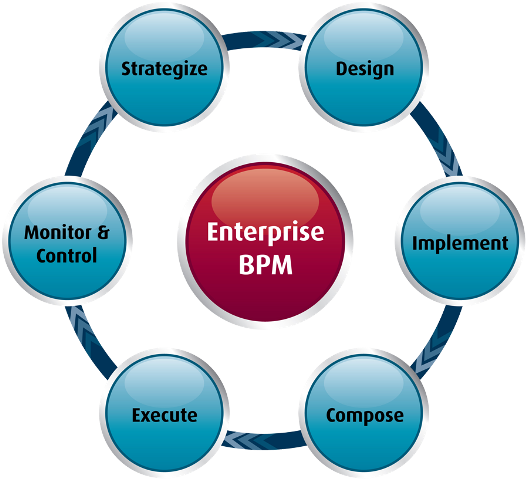
\includegraphics[width=0.6\textwidth]{bpm.png}
	\caption{Business Management cycle \cite{muede2}}
	\label{fig:anfang}
	\end{figure}
\subsubsection{Challenges of BPM \cite{bpmchall}}
\begin{itemize}
\item Lack of Business Case
\item Too Slow to React to the Business Change
\item Gap between the modelling and the implementation phases
\item Seen as a One Time Project 
\item Not Investing in Staff
\item Poorly Defined Measures of Success 
\end{itemize}
\subsubsection{BPML}
\subsubsection{BPEL}
\label{sec:bpel}
"BPEL (Business Process Execution Language) is an XML-based language that allows Web services in a service-oriented architecture to interconnect and share data.",\cite{bpelsearchsoa}. When using Webserivces, it also is often called WSBPEL. "Programmers use BPEL to define how a business process that involves web services will be executed. BPEL messages are typically used to invoke remote services, orchestrate process execution and manage events and exceptions.\\
BPEL is often associated with Business Process Management Notation (BPMN), a standard for representing business processes graphically. In many organizations, analysts use BPMN to visualize business processes and developers transform the visualizations to BPEL for execution.\\
BPEL was standardized by OASIS in 2004 after collaborative efforts to create the language by Microsoft, IBM and other companies.",\cite{bpelsearchsoa}.\\
\\
It therefore helps to produce code out of a graphical description, and there is no need to code it all out once again. Such systems should interact with other systems such as \gls{erp}-systems and without \gls{soa} it would be hard to realize. Using BPEL, smaller parts of an application can be easliy combined to a greater one. \cite[page 18]{soagoesreal}

\section{SOA Model if we need it}
The \gls{soa}-model has different layers. On the top level there is the Presentation Layer, which is the User Interface, which can be a normal Client Application as we know it but also a Fat Client. Then we speak of the Orchestration Layer, Where the flow of an Application is beeing a sequenz of certain services. In the Orchestration layer, a data transfer between these Services is possible as well. And then there comes the service layer, in which the Services are. In between there is some kind of integration Architecture, which would normally be an \gls{esb}. In the application layer, applications that already exists and Databases or systems are put. In the Visualized Infrastructure, the Hardware can be found. These layers can be seen in figure \ref{fig:soamodelarch}.
\begin{figure}[here!]
	\centering
	%\includegraphics[width=0.5\textwidth]{xxx}
	%\caption{EAI can also be seen a contributor of Service Orientation \cite[page 27]{soagoesreal}}
	\label{fig:soamodelarch}
	\end{figure}
	\FloatBarrier
\textbf{Orchestration}\\
Orchestration means, that a new Service can be build out of other Services. 
These other services can be of any kind (also external) and the communication between them is usually koordinated out from an central controlling instance. Orchestration is usually done using (WS-)BPEL as described closer in section \ref{sec:bpel}. This layer is also a reason why \gls{soa} is so flexible and why the systems must be loosely coupled. \cite[page 29]{soagoesreal}\\
\\
%mon petit grande 2
\textbf{SOA models}
There exist different SOA models, such as the OASIS model, The SOA Meta model of the W3C and each of the bigger companies such as IBM, SAP or Oracle have their own interpretation.

\section{JAX-WS}
SOAP-based Web services support in Java EE 5,6 and 7 is based on the Java API ....
site 112 grey book 

\newpage

\section{Implementation}
\subsection{ESB}
\label{sec:esb}
\subsection{RestFul Web Services}
RESTful web services are built to work best on the Web. RESTful applications use HTTP requests to post data (create and/or update), read data (e.g., make queries), and delete data. Thus, REST uses HTTP for all four CRUD (Create/Read/Update/Delete) operations. If you want to access resources like data and functionallaty in the REST architectural style you have to use Uniform Resource Identifiers which are typicaly links 
on the Web. The REST architectural style constrains an architecture to a client/server architecture and is designed to use a stateless communication protocol, typically HTTP. In the REST architecture style, clients and servers exchange representations of resources by using a standardized interface and protocol. //
The following principles encourage RESTful applications to be simple, lightweight, and fast:
\\
\begin{itemize}
\item Resource identification through URI: 
A RESTful web service exposes a set of resources that identify the targets of the interaction with its clients. Resources are identified by URIs, which provide a global addressing space for resource and service discovery.\\
\item Uniform interface: 
Resources are manipulated using a fixed set of four create, read, update, delete operations: PUT, GET, POST, and DELETE. PUT creates a new resource, which can be then deleted by using DELETE. GET retrieves the current state of a resource in some representation. POST transfers a new state onto a resource.\\
\item Self-descriptive messages: 
Resources are decoupled from their representation so that their content can be accessed in a variety of formats, such as HTML, XML, plain text, PDF, JPEG, JSON, and others. Metadata about the resource is available and used, for example, to control caching, detect transmission errors, negotiate the appropriate representation format, and perform authentication or access control. \\
\item Stateful interactions through hyperlinks:
Every interaction with a resource is stateless; that is, request messages are self-contained. Stateful interactions are based on the concept of explicit state transfer. Several techniques exist to exchange state, such as URI rewriting, cookies, and hidden form fields. State can be embedded in response messages to point to valid future states of the interaction.\\
\end{itemize}
\cite{RESTful}

=======
%TODO use the esb chapter
\subsection{Migration of legacy systems}
"Due to the frequency of change in business requirements and evolution in technology, the need
to evolve existing software systems is ever increasing. This results in demand for new methods
to support this process,in particular where the transition towards modern architectures is concerned.
SOAs are steadily becoming mainstream software engineering practice. Reports show that
more than 50 percent of large, newly developed applications and business processes designed during
the year 2007 used service-oriented architectures to some extent.",\cite{legacy}.
\\
\subsection{Protocols}
\subsubsection{XML}
XML stands for EXtensible Markup Language.XML was designed to describe data.
XML is a software- and hardware-independent tool for carrying information.\\
Besides HTML and XHTML the most widespread RESTful HTTP-enviroment.\\
Example:\\
\begin{lstlisting}
<?xml version="1.0" encoding="UTF-8"?>
<orders xmlns="http://example.com/schemas/ordermanagment">
  <order href="/orders/442820205">
    <customer>
  ...
    <customer>
  </order>
</orders>
\end{lstlisting}
Buch REST und HTTP Seite 83
\subsubsection{JSON}
The focus lies ,if compared to XML, in datastructure and not text.
Does not support namespaces and schemed based validation but is easier to understand
than XML.\\
Example:\\
\begin{lstlisting}
{"widget": {
    "debug": "on",
    "window": {
        "title": "Sample Konfabulator Widget",
        "name": "main_window",
        "width": 500,
        "height": 500
    },
    "image": { 
        "src": "Images/Sun.png",
        "name": "sun1",
        "hOffset": 250,
        "vOffset": 250,
        "alignment": "center"
    },
    "text": {
        "data": "Click Here",
        "size": 36,
        "style": "bold",
        "name": "text1",
        "hOffset": 250,
        "vOffset": 100,
        "alignment": "center",
        "onMouseUp": "sun1.opacity = (sun1.opacity / 100) * 90;"
    }
}}
\end{lstlisting}
todo{ better Example}
\subsubsection{SOAP}
SOAP was originally a shortcut for "Simple Object Access Protocol", but since it isn't simple 
and it isn't used to access object only the protocol was correct. Since version 1.2 the shortcut
was abolished and SOAP now stands for itself.
todo{Example + what is does}
SOA in der Praxis S 268
\subsubsection{WSDL}
Web Service Description Language is a XML based Interface communicationinterface description language
which is used to describe web services which are called by SOAP-Messages.
Currently there are two Versions:\\
1.1 : Which is used Worldwide and is supported by nearly every tool \\
2.0 : Brings some improvments but they are not relevant in the praxis\\

todo{ SOA in der Praxis S 263 Example}
\subsubsection{UUID}
"A UUID (Universal Unique Identifier) is a 128-bit number used to uniquely identify some object or entity on the Internet. Depending on the specific mechanisms used, a UUID is either guaranteed to be different or is, at least, extremely likely to be different from any other UUID generated until 3400 A.D.A guaranteed UUID contains a reference to the network address of the host that generated the UUID, a timestamp (a record of the precise time of a transaction), and a randomly generated component.A UUID is specified as part of the tModel data structure, which represents a service type (a generic representation of a registered service) in the UDDI (Universal Description, Discovery, and Integration) registry. This mechanism is used to discover Web services."\cite{UUID}

\section{Code Snippets}
Rest Servlet
\begin{lstlisting}
<?xml version="1.0" encoding="UTF-8"?>
<beans xmlns="http://www.springframework.org/schema/beans"
  xmlns:context="http://www.springframework.org/schema/context"
  xmlns:mvc="http://www.springframework.org/schema/mvc" xmlns:xsi="http://www.w3.org/2001/XMLSchema-instance"
  xmlns:p="http://www.springframework.org/schema/p"
  xsi:schemaLocation="
        http://www.springframework.org/schema/beans     
        http://www.springframework.org/schema/beans/spring-beans-4.0.xsd
        http://www.springframework.org/schema/context
        http://www.springframework.org/schema/context/spring-context-4.0.xsd
        http://www.springframework.org/schema/mvc
        http://www.springframework.org/schema/mvc/spring-mvc-4.0.xsd">
  <context:component-scan base-package="at.xion.watcher" />
  <mvc:annotation-driven />
</beans>
\end{lstlisting}
Web XML
\begin{lstlisting}
<?xml version="1.0" encoding="UTF-8"?>
<web-app xmlns:xsi="http://www.w3.org/2001/XMLSchema-instance" xmlns="http://xmlns.jcp.org/xml/ns/javaee" xsi:schemaLocation="http://xmlns.jcp.org/xml/ns/javaee http://xmlns.jcp.org/xml/ns/javaee/web-app_3_1.xsd" version="3.1">
  <display-name>WatcherTomcat</display-name>
  <servlet>
    <servlet-name>rest</servlet-name>
    <servlet-class> org.springframework.web.servlet.DispatcherServlet</servlet-class>
    <load-on-startup>1</load-on-startup>
  </servlet>
  <servlet-mapping>
    <servlet-name>rest</servlet-name>
    <url-pattern>/*</url-pattern>
  </servlet-mapping>
</web-app>
\end{lstlisting}
REST JAVA
\begin{lstlisting}
@RequestMapping("/addToken")
  public String addToken(@RequestParam(value = "token") String token, @RequestParam(value = "user") String user) throws IOException {
\end{lstlisting}
\begin{lstlisting}
@RequestMapping("/removeToken")
  public void removeToken(@RequestParam(value = "token") String token)
\end{lstlisting}
\section{Comparison}
\subsection{Pro and Contra of SOA}
\subsection{SOA VS. EAI}
"Differently than EAI, which deals with linking enterprise applications so they can communicate with one another (by means of an intelligent reasoning engine) and carry out 'batch' data transfers, is the service oriented architecture (\gls{soa}) that provides 'transactional' data transfers, with no third-party software required. SOA is different from the EAI approach in that it does not depend on a third-party solution." ,\cite{soadef}
\begin{figure}[here!]
	\centering
	%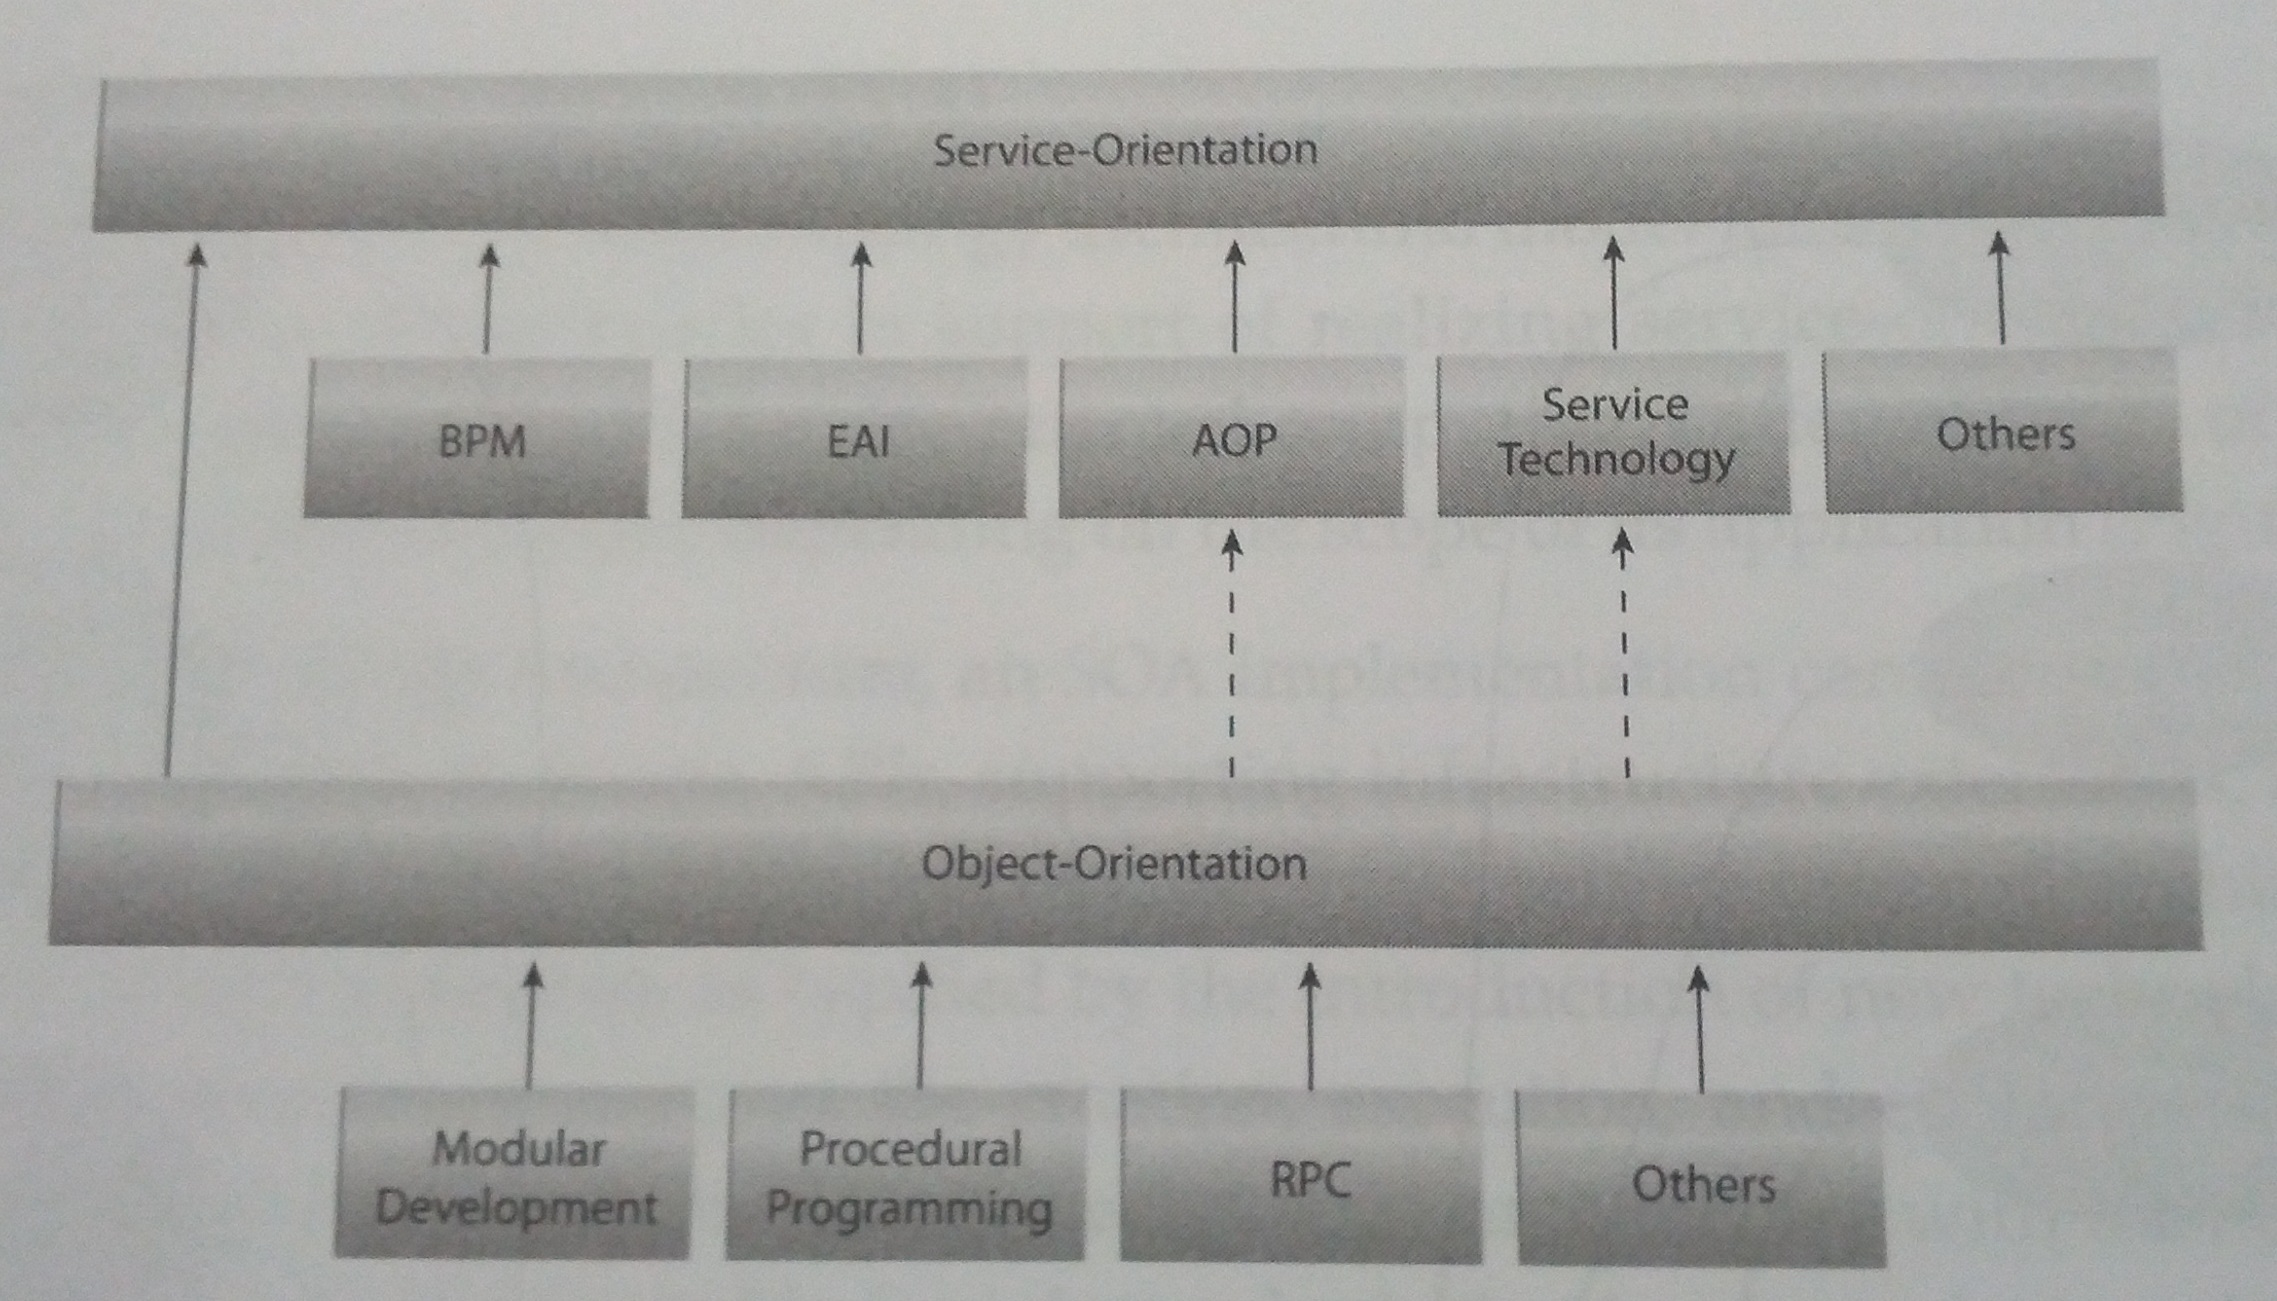
\includegraphics[width=0.5\textwidth]{b1_25.jpg}
	%\caption{EAI can also be seen a contributor of Service Orientation \cite[page 25]{book1}}
	\label{fig:eaipartofso}
	\end{figure}
\subsection{SOA VS. OOP}
\subsection{SOA VS. REST}



\section{Conclusion}
Whereas \gls{soa} can not be seen as an implementation but more as an design principle, it comes with many advantages. Using the Web-oriented approach and also putting Services and Business Processes into the focus, it leaves an very flexible IT-Infrastructure and leads to an cost efficient way of operating.\\
Nowadays, many of \gls{soa}'s principles are already used in what we declare as good software design, but still many companies have problems with applying the \gls{soa} Principles at a full extend. Often only parts of it get used, if even. This is mainly because changing an infrastructure is not that easy. \\


\section{If we need it!!}

\subsection{Implementation Topologies}
\subsubsection{Peer-to-peer}
The peer-to-peer (Figure \ref{fig:eai0}) implementation is not very useful. It is quite outdated and it is not really usable for modern systems.
There is practically no way to achieve any scalability and it gets complicated very soon. 
\subsubsection{Hub \& Spoke}
Messages get directed to an centralized unit, where they can be processed. (Figure \ref{fig:eai1}) This centralized unit can be a bottleneck though. 
\subsubsection{Bus}
Every service is connected to an service bus (\gls{esb}).(Figure \ref{fig:eai2}) The processing distribution in this case is very good. The bus-topology is therefore the most recommended one, because there is no bottleneck when comparing it to a Hub.
\begin{figure}[here!]
\centering
\begin{minipage}[h]{0.3\textwidth}
\centering
    %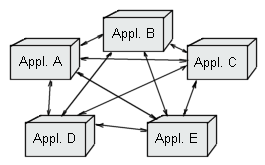
\includegraphics[width=1.0\textwidth]{eai0.png}
    %\caption{Star-topology \cite{thorstenhorn}}
    \label{fig:eai0}
\end{minipage}
\begin{minipage}[h]{0.3\textwidth}
\centering
    %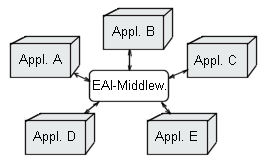
\includegraphics[width=1.0\textwidth]{eai1.png}
    %\caption{Hub-topology \cite{thorstenhorn}}
    \label{fig:eai1}
\end{minipage}
\begin{minipage}[h]{0.3\textwidth}
\centering
    %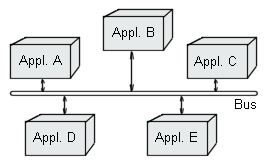
\includegraphics[width=1.0\textwidth]{eai2.png}
    %\caption{Bus-topology \cite{thorstenhorn}}
    \label{fig:eai2}
\end{minipage}
\end{figure}
\FloatBarrier

\listoftables
\listoffigures
\printglossaries
\subsection{Easy Bibliography}
\begin{thebibliography}{56}

\bibitem{te}
   \textbf{Who}, When\\
  \textit{url}
  \newline last used: dd.mm.yyyy, hh:mm


\bibitem{grau}
   \textbf{Who}, When\\
  \textit{url}
  \newline last used: dd.mm.yyyy, hh:mm
 
 
\bibitem{gruen}
   \textbf{Who}, When\\
  \textit{url}
  \newline last used: dd.mm.yyyy, hh:mm
 
 
\bibitem{echse}
   \textbf{Who}, When\\
  \textit{url}
  \newline last used: dd.mm.yyyy, hh:mm
 
  
\bibitem{soagoesreal}
   \textbf{Who}, When\\
  \textit{url}
  \newline last used: dd.mm.yyyy, hh:mm
    
 
\bibitem{esoa}
   \textbf{Who}, When\\
  \textit{url}
  \newline last used: dd.mm.yyyy, hh:mm
  
 
\bibitem{jweb}
   \textbf{Who}, When\\
  \textit{url}
  \newline last used: dd.mm.yyyy, hh:mm
    
  
   
 
\bibitem{service1}
   \textbf{Service},service-architecture.com \\
  \textit{http://www.service-architecture.com/articles/web-services/service.html}
  \newline last used: 03.02.2015, 13:39
     
     
     \bibitem{soaserviearch}
   \textbf{Service-Oriented Architecture (SOA) Definition},service-architecture.com \\
  \textit{http://www.service-architecture.com/articles/web-services/service-oriented\_architecture\_soa\_definition.html}
  \newline last used: 03.02.2015, 13:40
     
     
     \bibitem{soaitwissen}
   \textbf{SOA (service oriented architecture)},IT Wissen \\
  \textit{http://www.itwissen.info/definition/lexikon/service-oriented-architecture-SOA-SOA-Architektur.html}
  \newline last used: 03.02.2015, 13:50
     
     \bibitem{searchsoa}
   \textbf{service-oriented architecture (SOA) definition},Margaret Rouse \\
  \textit{http://searchsoa.techtarget.com/definition/service-oriented-architecture}
  \newline last used: 03.02.2015, 14:05

\bibitem{json}
  \textbf{JSON},json.com
  \textit{http://www.json.org/}
  \newline last used: 02.02.2015, 22:15

 
     \bibitem{soamaifesto}
   \textbf{The SOA Manifesto} \\
  \textit{http://www.soa-manifesto.org/default.html}
  \newline last used: 28.02.2015, 14:05


     \bibitem{bpelsearchsoa}
   \textbf{BPEL (Business Process Execution Language) definition},Margaret Rouse \\
  \textit{http://searchsoa.techtarget.com/definition/BPEL}
  \newline last used: 08.03.2015, 13:21

<<<<<<< HEAD
  \bibitem{legacy}
    \textbf{Migrating Legacy System to Service-Oriented Architecture },Carlos Matos\\
    \textit{http://kobv.de/opus4}
    \newline last used : 09.03.2015, 21:50

  \bibitem{RESTful}
    \textbf{What Are RESTful Web Services},Oracle
    \textit{http://docs.oracle.com/javaee/6/tutorial/doc/gijqy.html}
    \newline last used : 09.03.2015, 22:30

    \bibitem{UUID}
    \textbf{UUID (Universal Unique Identifier) definition},Margaret Rouse\\
    \textit{http://searchsoa.techtarget.com/definition/UUID}
    \newline last used : 09.03.2015, 23:55

=======
\bibitem{bpmdef}
   \textbf{Business Process Management (BPM)}, Margaret Rouse\\
  \emph{http://searchcio.techtarget.com/definition/business-process-management}
  \newline abgerufen am: 06.10.2014, 22:13
  

  \bibitem{bpmchall}
   \textbf{Top Ten Biggest Challenges to BPM Initiatives}, Pearl Zhu\\
  \emph{http://futureofcio.blogspot.co.at/2013/03/top-ten-biggest-challenges-to-bpm.html}
  \newline abgerufen am: 06.10.2014, 22:32
 
>>>>>>> df0ebff46426b848dc6953afa5b8d2e691223e1e
 
 \bibitem{muede2}
   \textbf{What is Business Process Management? }\\
  \emph{http://www.scc-co.com/enterprises-processes/}
  \newline abgerufen am: 06.10.2014, 22:04


  \bibitem{soadef}
   \textbf{Key differnces between ESB, EAI and SOA}\\
  \emph{www.innovativearchitects.com/KnowloedgeCenter/Business\%20Connectivity\%20and\%20Interoperability/ESB-EAI-SOA.aspx}
  \newline abgerufen am: 06.10.2014, 22:18


\bibitem{thorstenhorn}
   \textbf{Torsten Horn}\newline
  \emph{http://www.torsten-horn.de/techdocs/eai.htm}
  \newline abgerufen am: 05.10.2014, 20:25


%TODO haeee das is aus dem EAI Referat
    \bibitem{book1}
   \textbf{SOA with Java}, Thomas Erl \\
 	 ISBN: 0-13-385903-4
\end{thebibliography}
\end{document}
